\newlecture

\setcounter{chapter}{12}
\setcounter{section}{1}
%\def\textbookchapter{Chapter 12: Vector Calculus}
\def\coursetopicnumber{IV}
\def\topic{The Idea of a Line Integral} % this is the printed title
\def\shorttopic{Line integrals} % short topic
\def\textbookname{Active Calculus} % this is the corresponding textbook
\def\shorttextbookname{AC} % this is the short name for the book
\def\textbooksection{12.2} % corresponding textbook section
\def\textbooksectionurl{https://activecalculus.org/vector/S_Vector_IdeaLineIntegral.html} % URL for textbook section
\def\handoutday{} % this is the printed date

%%%%%%%%% DOCUMENT CONTENT STARTS BELOW

\thispagestyle{plain}
\topstuff
\section{\topic{} \booklink{}}
\label{sec:idea-line-integral}
\subsection{Motivation: Work}
From physics, we know that work = force $\cdot$ distance.

In Section \ref{sec:dot-product}, we saw that if $\vec{F}$ represents a constant force acting on an object moving in a straight line from point $P$ to point $Q$, then we have the displacement vector $\vec{d}=\vec{PQ}$ and the work done in moving the object from $P$ to $Q$ 
\[
    W=\phantom{\vec{F}\dotp\vec{d}.}
\] 
%\vspace{.3in}

This formula works as long as 
%\begin{multicols}{2}
\begin{itemize}
    \item $\vec{F}$ doesn't change; and 
    \item movement is in a straight line.
\end{itemize}
%\end{multicols}

\bigskip 

\subsubsection{Positive/negative/zero work}
Let $\theta$ be the angle between $\vec{F}$ and $\vec{d}$.

\begin{enumerate}
    \item Work is positive if $\theta<90^\circ$.\\
    \item Work is zero if $\theta=90^\circ$.\\
    \item Work is negative if $90^\circ<\theta\le 180^\circ$.\\
\end{enumerate}

\begin{framed}
    In other words, work is positive if the force applied is at least somewhat in the direction of movement; work is negative if the force applied is at least somewhat against the direction of movement; and work is zero if the force applied is perpendicular to the direction of motion.
\end{framed}

With vector fields, we can compute work for a changing force and any sort of movement. We will do so with a \emph{line integral}. Before we learn about line integrals, we'll recall some things about parametrizations.

\pagebreak 

\subsection{Parametrizations: descriptions of movement}
In Chapter 9, we saw how to parametrize motion using vector-valued functions.
\begin{itemize} 
    \item In Section \ref{sec:lines-and-planes}, we saw how to parametrize motion along a line. 
    \item In Section \ref{sec:vector-valued-functions}, we saw how to parametrize motion along a circle as well as along the graph of a function $y=f(x)$. We also saw how to reverse the direction and shift time with a parametrization.
\end{itemize}

Each parametrization is represented by a vector-valued function $\vec{r}(t)=\langle x(t),y(t)\rangle$ along with an interval of $t$ values. We view $\vec{r}(t)$ as a position vector, meaning an object is at the point $(x(t),y(t))$ at time $t$. As $t$ changes, the position changes and we have motion. In this way, we can graph $\vec{r}(t)$ and obtain a \emph{path}.

Typically, we write $\vec{r}(t)=\langle x(t),\, y(t)\rangle$ for a path in $\mathbb{R}^2$. Written with parametric equations, we have $x=x(t)$ and $y=y(t)$.

Similarly, we write $\vec{r}(t)=\langle x(t),\, y(t),\, z(t)\rangle$ for a path in $\mathbb{R}^3$. Written with parametric equations, we have $x=x(t)$, $y=y(t)$, and $z=z(t)$.

\begin{defn}[Smooth path]
    Suppose $\vec{r}(t)$ is a parametrization with $t$ in $[a,b]$ that describes a path $C$. The path $C$ is \emph{smooth} if, for all $t$ in $[a,b]$, $\vec{r}\,'(t)$ is continuous and $|\vec{r}\,'(t)|\ne0$.
\end{defn} 

\begin{ex}
    Let $P=(2,0)$ and $Q=(0,2)$.
    \begin{enumerate}
        \item Find and draw a parametrization for the line segment from $P$ to $Q$. Is this path smooth?
        \vfill 
        
        \item Find and draw a parametrization for the circular arc from $P$ to $Q$. Is this path smooth?
        \vfill
    \end{enumerate}
\end{ex}

\pagebreak

\subsection{Computing work in a force field}
Suppose $\vec{F}(x,y)$ represents a force applied to an object at the point $(x,y)$. If we have an object that moves from a point $P$ to a point $Q$, then there is a parametrization $\vec{r}(t)$ of the object's motion, for time $t$ in an interval $[a,b]$. As the object moves, it may experience different forces in terms of direction and magnitude. Our goal is to compute the work done as an object moves along its path in $\mathbb{R}^2$, from $t=a$ to $t=b$.

Here's the process:

%\begin{minipage}{.65\textwidth}
\begin{itemize}
    %\item Let $\vec{F}(x,y)$ represent a force on an object at the point $(x,y)$.
    %\item Let $\vec{r}(t)=\langle x(t),\, y(t)\rangle$ for $a\le t\le b$ describe the path of an object in the $xy$-plane. (We call $\vec{r}(t)$ a \emph{parametrization}.)
    %	\begin{itemize}
    %    \item Note that $\vec{r}(t)$ is a position vector, so at time $t$, our object is at the point $(x(t),y(t))$.
    %    \end{itemize}
    \item Split the interval $[a,b]$ up into $n$ intervals, each of length $\Delta t$: $[t_0,t_1]$, $[t_1,t_2]$, \dots, $[t_{n-1},t_n]$.
    \item At time $t_i$, the position of the object is $\vec{r}_i=\vec{r}(t_i)$. The force applied to the object at that moment is $\vec{F}(\vec{r}_i)$. The force is likely changing, but if $\Delta t$ is small, then the force is practically constant from $t_i$ to $t_{i+1}$.
    \item On the interval $[t_i,t_{i+1}]$, the object moves from $\vec{r}_i$ to $\vec{r}_{i+1}$. The movement might not be in a straight line, but if $\Delta t$ is small, then the motion from $t_i$ to $t_{i+1}$ is approximately a straight line. Let $\Delta\vec{r}_i$ be that straight line, so $\Delta\vec{r}_i=\vec{r}_{i+1}-\vec{r}_i$.
    \item We illustrate this with a picture from the textbook. (\href{https://activecalculus.org/vector/S_Vector_IdeaLineIntegral.html\#SS_Vector_IdeaLineIntegral_LineIntegrals}{Click here to see it in context.}) 
    %\footnote{
%    This image is from the textbook. To see it in context, see \url{https://activecalculus.org/vector/S_Vector_IdeaLineIntegral.html\#SS_Vector_IdeaLineIntegral_LineIntegrals}.
    %}
    %{Click here to see it in context.}}
    %illustrates this. 
    % Can't figure out how to avoid an error with the URL in the footnote.
    The path from $P$ to $Q$ is in black; the position at time $i$ is $\vec{r}_i$; the approximate motion at time $i$, $\Delta\vec{r}_i,$ is in blue; and the force at time $i$, $\vec{F}(\vec{r}_i)$, is in green.
    
    {\centering 
        \includegraphics[scale=.2]{images/fig_12_2_curve_vec_field.png}\label{img:textbook-vector-field}
    \par} 
    
    \item The work from $t=t_i$ to $t=t_{i+1}$ is then approximately $W_i \approx $% \vec{F}(\vec{r}(t_i))\dotp\vec{d}_i.\]
    \item Adding up the work for every interval, we obtain:
    \bigskip 
    
    \noindent $W \approx $ % \displaystyle \sum\limits_{i=0}^{n-1} W_i = $% 
    \bigskip 
    
    \item Our line segments will fit the path better if $\Delta t$ gets smaller and smaller. We can take a limit as $n$ goes to infinity to get an exact result. When that happens, we get
    \bigskip 
    
    \noindent $W = \displaystyle \phantom{\int\limits_a^b \vec{F}(\vec{r}(t))\dotp\vec{r}'(t)\dt.}$
    %\hspace{3in}$%\sum\limits_{i=1}^n \vec{F}\left(\vec{r}(t_i)\right)\dotp\left(\vec{r}(t_{i+1})-\vec{r}(t_i)\right).\]
\end{itemize}
\vfill 
%\end{minipage}
%\begin{minipage}{.3\textwidth}
%\end{minipage}

\pagebreak 

\subsection{Line integral definition}
The work calculation motivates the definition of a line integral along with some consequences.

\begin{defn}[Line integral of a vector field over a smooth path]
    Let $\vec{F}$ be a vector field, and let $C$ be a smooth path given by the parametrization $\vec{r}(t)$ for $t$ in $[a,b]$. 
    The \emph{line integral} of the vector field $\vec{F}$ over $C$ is denoted
    \[
        \phantom{\int\limits_C \vec{F}(\vec{r})\dotp \dif\vec{r}.} 
    \]
\end{defn}

\vspace{.8in}

Suppose we have two paths: $C_1$ starts at a point $P$ and ends at a point $Q$; and $C_2$ starts at a point $Q$ and ends at a point $R$. Then we can combine these paths to get a path $C$ that starts at $P$, goes through $Q$, and ends at $R$. Then\\
\[\hspace{-3in}\int\limits_C\vec{F}\dotp\dvr = \phantom{\int\limits_{C_1}\vec{F}\dotp\dvr + \int\limits_{C_2}\vec{F}\dotp\dvr.}\]
%To calculate the line integral of a vector field $\vec{F}$ over $C$, we can calculate the line integrals of $\vec{F}$ over $C_1$ and $C_2$ and then add the results.

%\vspace{.2in}

Suppose $C$ is a path from a point $P$ to a point $Q$. Let $-C$ denote the same path, but in reverse direction. I.e., $-C$ starts at $Q$ and ends at $P$. Then\\ 
\[\hspace{-3.8in}\int\limits_{-C}\vec{F}\dotp\dvr = \phantom{-\int\limits_C \vec{F}\dotp\dvr.}\]
%\vspace{.2in}

\begin{defn}[Piecewise smooth path, closed path, circulation]
    Suppose a continuous path $C$ is formed by combining paths $C_1, C_2, \dots, C_n$ for smooth paths $C_1,C_2,\dots,C_n$. We say $C$ is a \emph{piecewise smooth path}.
    
    A path that starts and ends at the same point is called a \emph{closed path}. \emph{Circulation} is the line integral of a vector field over a closed path.
\end{defn}

\begin{ex}
    Draw the path $C$ consisting of straight line segments from $(1,0)$ to $(4,0)$ to $(4,5)$ to $(1,0)$. Draw $C$. Is $C$ piecewise smooth? Is $C$ a closed path? For some vector field $\vec{F}(x,y)$, write $\int\limits_C \vec{F}\cdot\dvr$ as a sum of line integrals.
\end{ex}

\pagebreak 

\subsection{Definite integral visualization}
Before we learn how to compute line integrals (which we'll do in Section~\ref{sec:compute-line-integral}), we need to understand how to visualize them. Let's go back to understand how to visualize definite integrals.

\begin{ex}
    For each of the following, draw the graph of a continuous non-constant function $f(x)$ on $[1,6]$ that cross the $x$-axis at least once and satisfies the given property.
    \begin{multicols}{3} 
        \begin{enumerate}
            \item $\int\limits_1^{6}f(x)\dx>0$;
            \item $\int\limits_1^{6}f(x)\dx<0$;
            \item $\int\limits_1^{6}f(x)\dx=0$;
        \end{enumerate}
    \end{multicols}
\end{ex}

\vfill

\subsection{Line integral visualization}
%Quite often, for a function $f(x)$ graphed on an interval $[a,b]$, we can look at the graph and determine whether the definite integral is positive, negative, or zero. Now we'll see how to understand whether a given line integral is positive, negative or zero.

Just as a definite integral is an infinite sum of areas of rectangles, a line integral is an infinite sum of dot products. Each dot product involves a vector from the vector field $\vec{F}$ and a direction vector from our parametrization $\vec{r}(t)$. As we know, $\vec{r}(t)$ describes motion through the vector field $\vec{F}$.
\begin{itemize}
    \item Whenever motion is in the direction of a vector field, the dot product is positive. This makes a positive contribution to the line integral.
    \item The smaller the angle between the direction of motion and the direction of the vector field, the greater the positive contribution. (Contribution is maximized when they're in exactly the same direction.)
    \item Whenever motion is against the direction of a vector field, the dot product is negative. This makes a negative contribution to the line integral.
    \item The smaller the angle between the direction of motion and the negative of the direction of the vector field, the greater the negative contribution. (Contribution is negatively maximized when they're in exactly opposite directions.)
    \item Whenever motion is in a direction orthogonal to a vector field, the dot product is zero.
\end{itemize}
Finally, larger vectors in a vector field amplify contributions -- they make positive contributions more positive, and they make negative contributions more negative.

\pagebreak 

\begin{framed}
    \noindent If a path $C$ is only ever in the direction of a vector field $\vec{F}$, the line integral is positive.
    
    \noindent If a path $C$ is only ever against the direction of a vector field $\vec{F}$, the line integral is negative.
    
    \noindent If a path $C$ is always orthogonal to a vector field, then the line integral  is zero.
\end{framed}

\begin{ex}
    \begin{enumerate} 
        \item In $\vec{F}$ below, draw paths $C_1$ and $C_2$ for which $\displaystyle\int\limits_{C_1}\vec{F}\dotp\dvr>0$ and $\displaystyle\int\limits_{C_2}\vec{F}\dotp\dvr<0$.
        \\
        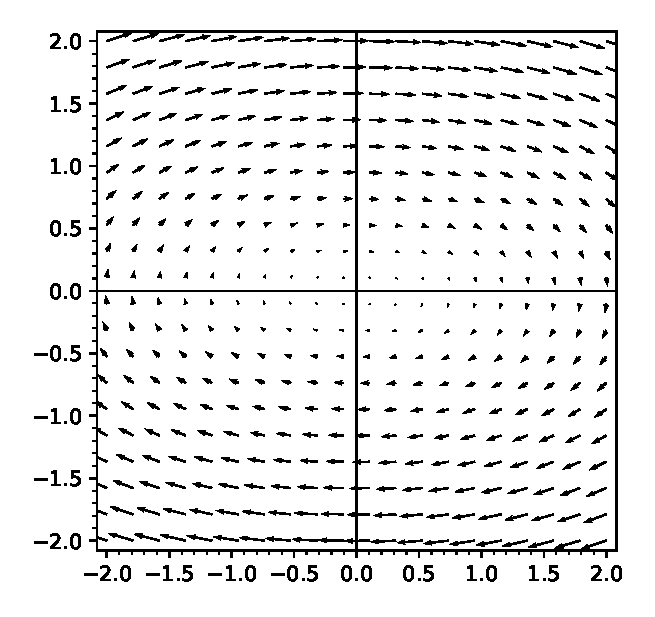
\includegraphics[scale=.9]{images/vector-field-to-draw-on-2.eps}\label{img:sage-vector-field-3}
        
        \item In $\vec{G}$ below, draw paths $C_1, C_2, C_3$ for which $\displaystyle\int\limits_{C_1}\vec{G}\dotp\dvr>\displaystyle\int\limits_{C_2}\vec{G}\dotp\dvr>0$ and $\displaystyle\int\limits_{C_3}\vec{G}\dotp\dvr=0$. 
        \\
        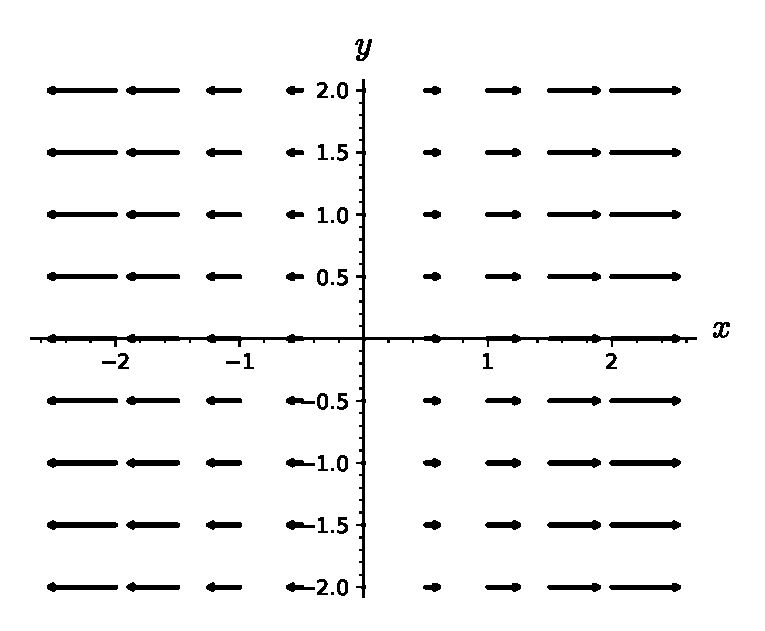
\includegraphics[scale=.8]{images/vector-field-to-draw-on-1.eps}
    \end{enumerate}
\end{ex}


